Structural assessment of the inflatable configuration has been performed by an estimation of internal forces. This is an essential step in the design of an inflatable aeroshell, since a force estimation:
\begin{itemize}
\item Is required to estimate the inflation pressure to maintain its structural integrity and aerodynamic shape under peak aerodynamic loading
\item Allows to identify whether loads allow for concept structural design within state-of-the-art material capabilities
\item Yields the loads at the structural interface between the inflatable aeroshell and the rigid centerbody
\item Gives an impression of the effect of changing design parameters on concept structural performance
\end{itemize}

Forces are estimated for an inflatable structure that is aerodynamically loaded, as follows from vehicle trajectory analysis in Chapter \ref{ch:XXX}, in its deployed condition. An interface with the aerodynamic analysis, performed in Chapter \ref{ch:XXX}, yields the optimized aeroshell shape as a baseline for the structural model used.

\subsubsection{Approach outline}
To meet the purposes of structural assessment of the inflatable configuration, force estimation is performed by a two-dimensional truss analysis on a simplified geometry. This geometry relies on the aerodynamic aeroshell shape, optimized in Chapter \ref{ch:XXX}, to define its outer shape. This shape is effected by a number of toroids \gls{sym:N}, held together by radial straps, running along the surface of the inflatable. 

Adjoining toroids are connected at three locations: by a radial strap along the forward side of the aeroshell (impinged by the flow), a radial strap running along the aft side of the aeroshell and at their direct contact surface. In reality, as in the stacked toroid configuration used for NASAs \gls{irve} \cite{Lindell2006}, the contact surface of adjoining toroids is a straight wall, while top and bottom surfaces are of circular shape. This shape is the result of the internally applied pressure: equal but oppositely directed pressures effect a straight interface between toroids and toroids adapt to the unbalanced pressure in top and bottom surfaces through energy minimization by taking a circular shape.

Simplification was performed to realize a structurally determinate problem results by modelling toroids as diamonds. The orientation of the diamonds is defined by the half-cone angle \gls{sym:theta}, allowed to vary over its radius and circumference per toroid, and their shape by a fixed width \gls{sym:w} and varying height \gls{sym:h}, to allow for a tapered structure. Nodes are designated as the corners of each diamond and connecting members have been numbered. The numbering convention and dimensions are illustrated in Figure \ref{fig:TC}. 


\begin{figure}[h]
	\centering
	\begin{subfigure}[b]{0.49\textwidth}
	\centering
	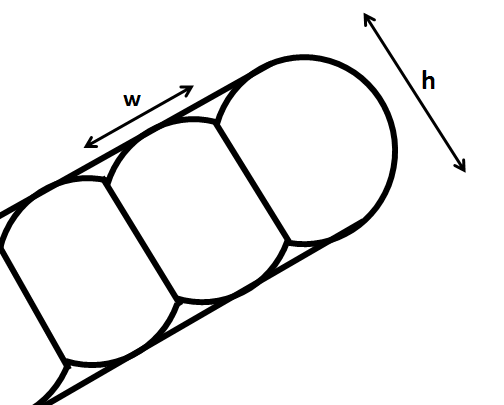
\includegraphics[width=1.0\textwidth]{./Figure/Structure/ToroidConfig.png}
	\caption{Actual toroid layout} 
	\label{fig:TC1}
	\end{subfigure}
	\begin{subfigure}[b]{0.49\textwidth}
	\centering
	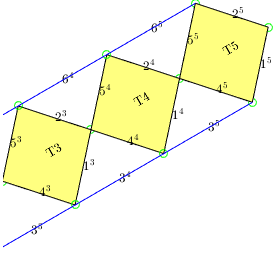
\includegraphics[width=1.0\textwidth]{./Figure/Structure/ToroidConfig2.png}
	\caption{Simplified truss model} 
	\label{fig:TC2}
	\end{subfigure}
	\caption{}
	\label{fig:TC}
\end{figure}

Force estimation is performed in a two-dimensional plane representing a cross-sectional slice, of an infinitesimal angle, of the sphere cone. Each toroid is loaded externally by an aerodynamic force applied perpendicular to its width \gls{sym:w} at its forward node (placed directly in the flow). The aerodynamic force is the resultant of the limit aerodynamic pressure $\gls{sym:q}_{limit}$, assumed constant for each toroid, multiplied by toroid width \gls{sym:w} to represent its working area. The limit aerodynamic pressure is determined from the peak dynamic pressure by multiplying with a \acrfull{fos}, thereby taking into account a contingency for structural design. The \gls{fos} is XXX????XXX??XXX. 

In addition to the aerodynamic pressure acting on the inflatable forward surface, movables (e.g. flaps) at the edge of the aeroshell are taken into account, where present, as a point load, of prescribed magnitude by control considerations following from Chapter \ref{ch:XXX}, directed perpendicular to the flap deployed surface area.

As input forces are in Newtons per meter, being the product of a pressure over a length, forces should technically be designated as forces per unit length or running loads. Hereafter, all references to forces in this section are in fact references to running loads. To calculate forces from running loads, these should be multiplied with the circumference over which they act.

On the basis of these external forces, estimation is performed by a truss analysis. By requiring force equilibrium in two orthogonal directions within the plane, internal forces in each of the members 1 to 6 for the \gls{sym:N} toroids are determined. This system of equations is solved from the free end (outboard) to the pinned end (inboard) where the inflatable is connected to the centerbody. At this location, reaction forces in two orthogonal directions are determined at the two attachment points, forward and aft.

The decreasing circumference over which forces act going from outboard to inboard in each two-dimensional slice, inherent to the sphere cone design, effects a proportional increase in running loads. This increase is proportional to the decrease in diameter, via the circumference, and thereby member forces are scaled by the ratio of radial distances, with respect to the centerbody longitudinal axis, of the nodes they connect.

After this first iteration, internal pressure is to be taken into account. 
